\documentclass{article}
\usepackage{graphicx}
\usepackage{amsmath}
\usepackage{tikz}
\usepackage{qtree}
\usetikzlibrary{calc,shapes.multipart,chains,arrows}
\graphicspath{ {./images/} }
\title{Modelling with Graphs Summative }
\begin{document}
\maketitle
\newpage
\section*{A.3}
\subsection*{A.3.1}
To transform problem A.3 into a graph colouring problem , the problem is represented as a graph where:
\newline
Nodes = individual classes $(C_1,..., C_7)$
\newline
Edges = classes with at least one shared student (eg. "Amy" in $C_1$ and $C_5$)
\newline
Colour = A timeslot
\newline
A representation of the graph as an adjacency matrix is:
\newline
\begin{center}
$\begin{pmatrix}
   0&1&1&0&1&1&0\\
   1&0&1&0&0&1&1\\
   1&1&0&0&0&1&0\\
   0&0&0&0&1&1&0\\
   1&0&0&1&0&1&1\\
   1&1&1&1&1&0&0\\
   0&1&0&0&1&0&0\\
\end{pmatrix}$
\end{center}
An example graph would be:
\newline
\begin{center}
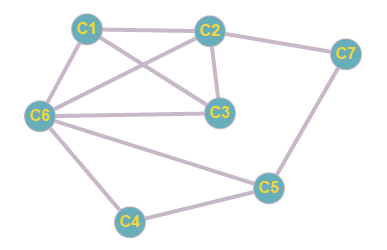
\includegraphics{a31NC}
\newline
\end{center}
The solution to the problem is the answer to the question, can the graph be coloured in at most 4 colours?
\newline
This will solve the problem because if the graph can be coloured so that no neighbouring nodes have the same timeslot then the student can physially attend every class, and by doing it in at most 4 colours means there are sufficient time slots.
\newline
An example colouring of the above graph would be:
\begin{center}
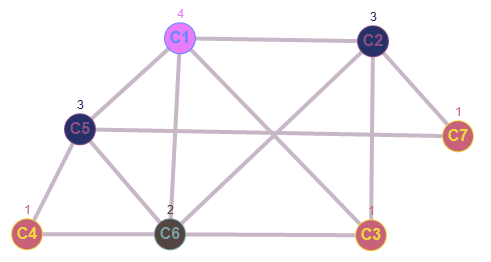
\includegraphics{a31C}
\end{center}
\subsection*{A.3.2}
As there are currently no visited nodes, the algorithm will first visit node $C_1$.
\begin{center}
Visited - $C_1$
\newline
Adjacent - $C_2,C_3,C_5,C_6$
\newline
\end{center}
Visit $C_2$
\begin{center}
Visited - $C_1,C_2$
\newline
Adjacent - $C_3,C_5,C_6,C_7$
\newline
\end{center}
Visit $C_3$
\begin{center}
Visited - $C_1,C_2,C_3$
\newline
Adjacent - $C_5,C_6,C_7$
\newline
\end{center}
Visit $C_6$
\begin{center}
Visited - $C_1,C_2,C_3,C_6$
\newline
Adjacent - $C_5,C_7$
\end{center}
Visit $C_4$
\begin{center}
Visited - $C_1,C_2,C_3,C_6,C_4$
\newline
Adjacent - $C_5,C_7$
\end{center}
Visit $C_5$
\begin{center}
Visited - $C_1,C_2,C_3,C_6,C_4,C_5$
\newline
Adjacent - $C_7$
\newline
\end{center}
Visit $C_7$
\begin{center}
Visited - $C_1,C_2,C_3,C_6,C_4,C_5,C_7$
\newline
\end{center}
Order in which the algorithm visits the vertices to find a proper colouring is:
\newline
\begin{center}
$C_1,C_2,C_3,C_6,C_4,C_5,C_7$
\end{center}
\subsection*{A.3.3}
The colours the algorithm assigns to each vertex are below:
\begin{center}
\begin{tabular}{ |c|c| }
\hline
Vertex & Colour \\
\hline
$C_1$  & 1      \\
$C_2$  & 2      \\
$C_3$  & 3      \\
$C_4$  & 1      \\
$C_5$  & 2      \\
$C_6$  & 4      \\
$C_7$  & 1       \\
\hline
\end{tabular}
\end{center}
\subsection*{A.3.4}
The chromatic number of G, $\chi$G, is 4 because it the minimum number of colours needed to properly colour G is 4.

\section*{B.2}
\subsection*{B.2.1}
The adjacency matrix for the graph is below:
\newline
\begin{center}
$\begin{pmatrix}
   0&1&1&1&1&0&0 \\
   1&0&0&0&0&1&1 \\
   1&0&0&0&0&0&1 \\
   1&0&0&0&0&0&1 \\
   1&0&0&0&0&1&0 \\
   0&1&0&0&1&0&0 \\
   0&1&1&1&0&0&0 \\
\end{pmatrix}$
\end{center}
And the adjacency linked list is below:
\newline
1:
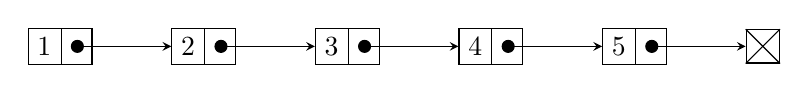
\begin{tikzpicture}[list/.style={rectangle split, rectangle split parts=2,
    draw, rectangle split horizontal}, >=stealth, start chain]
    \node[list,on chain] (A) {1};
  \node[list,on chain] (B) {2};
  \node[list,on chain] (C) {3};
 \node[list,on chain] (D) {4};
 \node[list,on chain] (E) {5};
  \node[on chain,draw,inner sep=6pt] (F) {};
  \draw (F.north east) -- (F.south west);
  \draw (F.north west) -- (F.south east);
  \draw[*->] let \p1 = (A.two), \p2 = (A.center) in (\x1,\y2) -- (B);
  \draw[*->] let \p1 = (B.two), \p2 = (B.center) in (\x1,\y2) -- (C);
  \draw[*->] let \p1 = (C.two), \p2 = (C.center) in (\x1,\y2) -- (D);
\draw[*->] let \p1 = (D.two), \p2 = (D.center) in (\x1,\y2) -- (E);
\draw[*->] let \p1 = (E.two), \p2 = (E.center) in (\x1,\y2) -- (F);
\end{tikzpicture}
\newline
2:
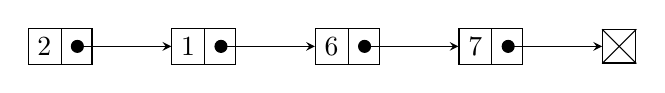
\begin{tikzpicture}[list/.style={rectangle split, rectangle split parts=2,
    draw, rectangle split horizontal}, >=stealth, start chain]
   \node[list,on chain] (A) {2};
  \node[list,on chain] (B) {1};
  \node[list,on chain] (C) {6};
 \node[list,on chain] (D) {7};
  \node[on chain,draw,inner sep=6pt] (E) {};
  \draw (E.north east) -- (E.south west);
  \draw (E.north west) -- (E.south east);
  \draw[*->] let \p1 = (A.two), \p2 = (A.center) in (\x1,\y2) -- (B);
  \draw[*->] let \p1 = (B.two), \p2 = (B.center) in (\x1,\y2) -- (C);
  \draw[*->] let \p1 = (C.two), \p2 = (C.center) in (\x1,\y2) -- (D);
\draw[*->] let \p1 = (D.two), \p2 = (D.center) in (\x1,\y2) -- (E);
\end{tikzpicture}
\newline
3:
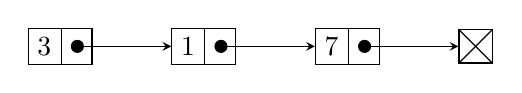
\begin{tikzpicture}[list/.style={rectangle split, rectangle split parts=2,
    draw, rectangle split horizontal}, >=stealth, start chain]
   \node[list,on chain] (A) {3};
  \node[list,on chain] (B) {1};
	\node[list,on chain] (C) {7};
  \node[on chain,draw,inner sep=6pt] (D) {};
  \draw (D.north east) -- (D.south west);
  \draw (D.north west) -- (D.south east);
  \draw[*->] let \p1 = (A.two), \p2 = (A.center) in (\x1,\y2) -- (B);
  \draw[*->] let \p1 = (B.two), \p2 = (B.center) in (\x1,\y2) -- (C);
  \draw[*->] let \p1 = (C.two), \p2 = (C.center) in (\x1,\y2) -- (D);
\end{tikzpicture}
\newline
4:
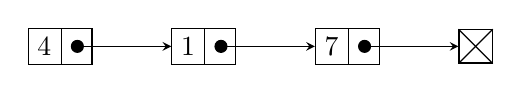
\begin{tikzpicture}[list/.style={rectangle split, rectangle split parts=2,
    draw, rectangle split horizontal}, >=stealth, start chain]
   \node[list,on chain] (A) {4};
  \node[list,on chain] (B) {1};
	\node[list,on chain] (C) {7};
  \node[on chain,draw,inner sep=6pt] (D) {};
  \draw (D.north east) -- (D.south west);
  \draw (D.north west) -- (D.south east);
  \draw[*->] let \p1 = (A.two), \p2 = (A.center) in (\x1,\y2) -- (B);
  \draw[*->] let \p1 = (B.two), \p2 = (B.center) in (\x1,\y2) -- (C);
  \draw[*->] let \p1 = (C.two), \p2 = (C.center) in (\x1,\y2) -- (D);
\end{tikzpicture}
\newline
5:
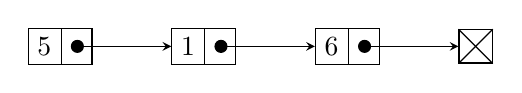
\begin{tikzpicture}[list/.style={rectangle split, rectangle split parts=2,
    draw, rectangle split horizontal}, >=stealth, start chain]
   \node[list,on chain] (A) {5};
  \node[list,on chain] (B) {1};
	\node[list,on chain] (C) {6};
  \node[on chain,draw,inner sep=6pt] (D) {};
  \draw (D.north east) -- (D.south west);
  \draw (D.north west) -- (D.south east);
  \draw[*->] let \p1 = (A.two), \p2 = (A.center) in (\x1,\y2) -- (B);
  \draw[*->] let \p1 = (B.two), \p2 = (B.center) in (\x1,\y2) -- (C);
  \draw[*->] let \p1 = (C.two), \p2 = (C.center) in (\x1,\y2) -- (D);
\end{tikzpicture}
\newline
6:
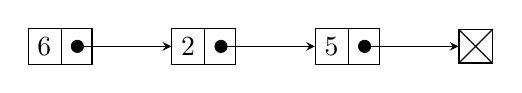
\begin{tikzpicture}[list/.style={rectangle split, rectangle split parts=2,
    draw, rectangle split horizontal}, >=stealth, start chain]
   \node[list,on chain] (A) {6};
  \node[list,on chain] (B) {2};
	\node[list,on chain] (C) {5};
  \node[on chain,draw,inner sep=6pt] (D) {};
  \draw (D.north east) -- (D.south west);
  \draw (D.north west) -- (D.south east);
  \draw[*->] let \p1 = (A.two), \p2 = (A.center) in (\x1,\y2) -- (B);
  \draw[*->] let \p1 = (B.two), \p2 = (B.center) in (\x1,\y2) -- (C);
  \draw[*->] let \p1 = (C.two), \p2 = (C.center) in (\x1,\y2) -- (D);
\end{tikzpicture}
\newline
7:
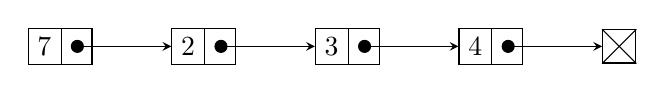
\begin{tikzpicture}[list/.style={rectangle split, rectangle split parts=2,
    draw, rectangle split horizontal}, >=stealth, start chain]
   \node[list,on chain] (A) {7};
  \node[list,on chain] (B) {2};
  \node[list,on chain] (C) {3};
 \node[list,on chain] (D) {4};
  \node[on chain,draw,inner sep=6pt] (E) {};
  \draw (E.north east) -- (E.south west);
  \draw (E.north west) -- (E.south east);
  \draw[*->] let \p1 = (A.two), \p2 = (A.center) in (\x1,\y2) -- (B);
  \draw[*->] let \p1 = (B.two), \p2 = (B.center) in (\x1,\y2) -- (C);
  \draw[*->] let \p1 = (C.two), \p2 = (C.center) in (\x1,\y2) -- (D);
\draw[*->] let \p1 = (D.two), \p2 = (D.center) in (\x1,\y2) -- (E);
\end{tikzpicture}
\subsection*{B.2.2}
The depth-first search tree for the graph in question B.2.1 is below:
\begin{center}
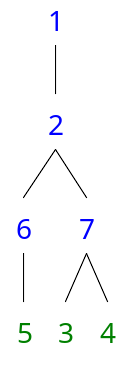
\includegraphics{dfsTree}
\end{center}
The table for when the in which the vertices are reached for the first time and he order in which the vertices become dead ends is below:
\begin{center}
\begin{tabular}{ |c|c|c|c|c|c|c|c|}
\hline
-&1&2&3&4&5&6&7     \\
\hline
On&1&2&6&7&4&3&5   \\
Off&7&6&3&4&1&2&5	 \\
\hline
\end{tabular}
\end{center}
\subsection*{2.3}
The graph with the addition of the weights is below:
\newline
\begin{center}
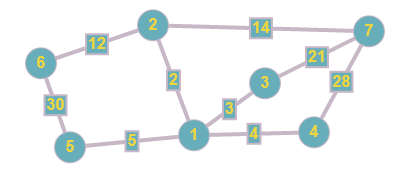
\includegraphics{b23W}
\end{center}
As Kruskal's algorithm runs it firsts adds the edge with the smallest weight to the tree, which is the edge between vertices '1' and '2' with weight 2. 
\newline
\begin{center}
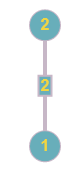
\includegraphics{b231}
\end{center}
Secondly, it adds the edge between '1' and '3' with weight 3.
\newline
\begin{center}
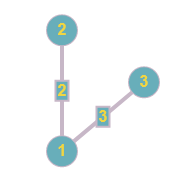
\includegraphics{b232}
\end{center}
Then, the algorithm will add the next smallest edge, the edge between '1' and '4' with weight 4.
\newline
\begin{center}
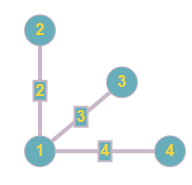
\includegraphics{b233}
\end{center}
The next edge added is the node between '1' and '5' with weight 5.
\newline
\begin{center}
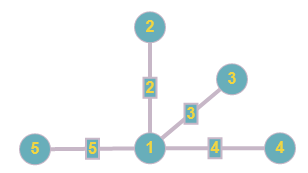
\includegraphics{b234}
\end{center}
Then, the algorithm will add the edge between '2' and '6' with weight 12.
\newline
\begin{center}
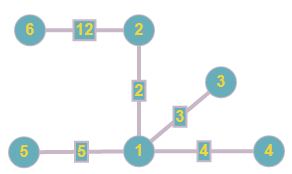
\includegraphics{b235}
\end{center}
The algorithm then finds the next smallest edge, the edge between '2' and '7' with weight 14 and adds it.
\newline
\begin{center}
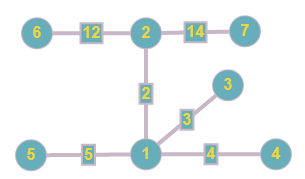
\includegraphics{b236}
\end{center}
The algorithm then looks at the next smallest edge, which is the edge between '3' and '7' which has a weight of 21. However this will not be added as it would create a cycle, '1,2,7,3,1'. 
\newline
\begin{center}
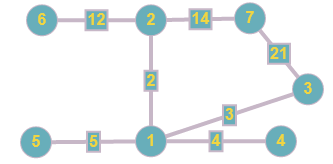
\includegraphics{b23c1}
\end{center}
The next edge the algorithm looks at is the edge between '4' and '7' which has weight 28. This will not be added as it would create a cycle '1,2,7,4,1'.
\begin{center}
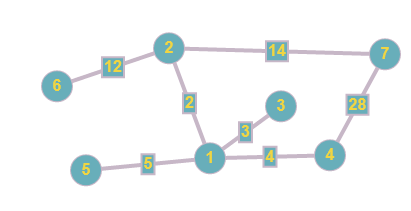
\includegraphics{b237}
\end{center}
Finally the algorithm looks at the edge between '5' and '6' which has a weight of 30. However this is not added as it would create a cycle, '1,2,6,5,1'.
\newline
\begin{center}
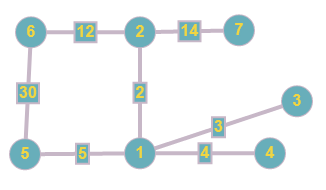
\includegraphics{b23c2}
\end{center}
So the final order minimum spanning tree is:
\begin{center}
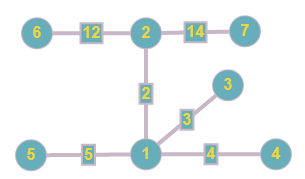
\includegraphics{b236}
\end{center}
With total weight (cost) is 40.
\end{document}